\documentclass[12pt,a4paper]{article}

%\usepackage[left=1.5cm,right=1.5cm,top=1cm,bottom=2cm]{geometry}
\usepackage[in, plain]{fullpage}
\usepackage{array}
%\usepackage{../../pas-math}
\usepackage{../../moncours}





%-------------------------------------------------------------------------------
%          -Packages nécessaires pour écrire en Français et en UTF8-
%-------------------------------------------------------------------------------
\usepackage[utf8]{inputenc}
\usepackage[frenchb]{babel}
\usepackage{numprint}
\usepackage[T1]{fontenc}
%\usepackage{lmodern}
\usepackage{textcomp}
\usepackage[french, boxed]{algorithm2e}


%-------------------------------------------------------------------------------

%-------------------------------------------------------------------------------
%                          -Outils de mise en forme-
%-------------------------------------------------------------------------------
\usepackage{hyperref}
\hypersetup{pdfstartview=XYZ}
%\usepackage{enumerate}
\usepackage{graphicx}
\usepackage{multicol}
\usepackage{tabularx}
\usepackage{multirow}
\usepackage{color}
\usepackage{eurosym}


\usepackage{anysize} %%pour pouvoir mettre les marges qu'on veut
%\marginsize{2.5cm}{2.5cm}{2.5cm}{2.5cm}

\usepackage{indentfirst} %%pour que les premier paragraphes soient aussi indentés
\usepackage{verbatim}
\usepackage{enumitem}
\usepackage[usenames,dvipsnames,svgnames,table]{xcolor}

\usepackage{variations}

%-------------------------------------------------------------------------------


%-------------------------------------------------------------------------------
%                  -Nécessaires pour écrire des mathématiques-
%-------------------------------------------------------------------------------
\usepackage{amsfonts}
\usepackage{amssymb}
\usepackage{amsmath}
\usepackage{amsthm}
\usepackage{tikz}
\usepackage{xlop}
\usepackage[output-decimal-marker={,}]{siunitx}
%-------------------------------------------------------------------------------



%-------------------------------------------------------------------------------


%-------------------------------------------------------------------------------
%                    - Mise en forme avancée
%-------------------------------------------------------------------------------

\usepackage{ifthen}
\usepackage{ifmtarg}


\newcommand{\ifTrue}[2]{\ifthenelse{\equal{#1}{true}}{#2}{$\qquad \qquad$}}

%\newcommand{\kword}[1]{\textcolor{red}{\underline{#1}}}
%-------------------------------------------------------------------------------

%-------------------------------------------------------------------------------
%                     -Mise en forme d'exercices-
%-------------------------------------------------------------------------------
%\newtheoremstyle{exostyle}
%{\topsep}% espace avant
%{\topsep}% espace apres
%{}% Police utilisee par le style de thm
%{}% Indentation (vide = aucune, \parindent = indentation paragraphe)
%{\bfseries}% Police du titre de thm
%{.}% Signe de ponctuation apres le titre du thm
%{ }% Espace apres le titre du thm (\newline = linebreak)
%{\thmname{#1}\thmnumber{ #2}\thmnote{. \normalfont{\textit{#3}}}}% composants du titre du thm : \thmname = nom du thm, \thmnumber = numéro du thm, \thmnote = sous-titre du thm

%\theoremstyle{exostyle}
%\newtheorem{exercice}{Exercice}
%
%\newenvironment{questions}{
%\begin{enumerate}[\hspace{12pt}\bfseries\itshape a.]}{\end{enumerate}
%} %mettre un 1 à la place du a si on veut des numéros au lieu de lettres pour les questions 
%-------------------------------------------------------------------------------

%-------------------------------------------------------------------------------
%                    - Mise en forme de tableaux -
%-------------------------------------------------------------------------------

\renewcommand{\arraystretch}{1.7}

\setlength{\tabcolsep}{1.2cm}

%-------------------------------------------------------------------------------



%-------------------------------------------------------------------------------
%                    - Racourcis d'écriture -
%-------------------------------------------------------------------------------
%Droites
\newcommand{\dte}[1]{$(#1)$}
\newcommand{\fig}[1]{figure $#1$}
\newcommand{\sym}{symétrique}
\newcommand{\syms}{symétriques}
\newcommand{\asym}{axe de symétrie}
\newcommand{\asyms}{axes de symétrie}
\newcommand{\seg}[1]{$[#1]$}
\newcommand{\monAngle}[1]{$\widehat{#1}$}
\newcommand{\bissec}{bissectrice}
\newcommand{\mediat}{médiatrice}
\newcommand{\ddte}[1]{$[#1)$}


% Angles orientés (couples de vecteurs)
\newcommand{\aopp}[2]{(\vec{#1}, \vec{#2})} %Les deuc vecteurs sont positifs
\newcommand{\aopn}[2]{(\vec{#1}, -\vec{#2})} %Le second vecteur est négatif
\newcommand{\aonp}[2]{(-\vec{#1}, \vec{#2})} %Le premier vecteur est négatif
\newcommand{\aonn}[2]{(-\vec{#1}, -\vec{#2})} %Les deux vecteurs sont négatifs

%Ensembles mathématiques
\newcommand{\naturels}{\mathbb{N}} %Nombres naturels
\newcommand{\relatifs}{\mathbb{Z}} %Nombres relatifs
\newcommand{\rationnels}{\mathbb{Q}} %Nombres rationnels
\newcommand{\reels}{\mathbb{R}} %Nombres réels
\newcommand{\complexes}{\mathbb{C}} %Nombres complexes


%Intégration des parenthèses aux cosinus
\newcommand{\cosP}[1]{\cos\left(#1\right)}
\newcommand{\sinP}[1]{\sin\left(#1\right)}


%Probas stats
\newcommand{\stat}{statistique}
\newcommand{\stats}{statistiques}


\newcommand{\homo}{homothétie}
\newcommand{\homos}{homothéties}


\newcommand{\mycoord}[3]{(\textcolor{red}{\num{#1}} ; \textcolor{Green}{\num{#2}} ; \textcolor{blue}{\num{#3}})}
%-------------------------------------------------------------------------------

%-------------------------------------------------------------------------------
%                    - Mise en page -
%-------------------------------------------------------------------------------

\newcommand{\twoCol}[1]{\begin{multicols}{2}#1\end{multicols}}


\setenumerate[1]{font=\bfseries,label=\textit{\alph*})}
\setenumerate[2]{font=\bfseries,label=\arabic*)}


%-------------------------------------------------------------------------------
%                    - Elements cours -
%-------------------------------------------------------------------------------

%Correction d'exercice
\newcommand{\exoSec}[2]{\subsection*{Exercice #1 page #2}}
%-------------------------------------------------------------------------------
%                    - raccourcis d'écriture -
%-------------------------------------------------------------------------------

%Mise en évidence de termes clés
\newcommand{\mykw}[1]{\textcolor{red}{\underline{\textbf{#1}}}}

%Exercices
\newcommand{\exo}[2]{exercice #1 page #2}
\newcommand{\Exo}[2]{Exercice #1 page #2}






\date{}
\title{}

\graphicspath{{./img/}}

\begin{document}
	
	
\chap[num=4, color=blue]{Quel espace un gaz peut-il occuper ?}{Olivier FINOT, \today }	

\section{La forme des liquides et des solides}

\begin{myact}{1 page 124}
	\begin{enumerate}
		\item Non les glaçons n'ont pas la forme du récipient qui les contient.\pause
		\item Le liquide obtenu lorsque les glaçons ont fondu a la forme du récipient.\pause
		\item La surface libre du liquide est plane.\pause
		\item On peut saisir un glaçon avec ses doigts, mais pas de l'eau liquide.\pause
		\item Lorsqu'il est placé dans des récipients de forme différentes, un solide conserve sa forme.\pause
		\item Un solide a une forme propre parce qu'elle ne change pas.\pause
		\item Un liquide placé dans dans des récipients de formes différentes prend la forme de ces récipients.\pause
		\item Le fil à plomb indique la direction verticale, donc le petit côté de l'équerre indique la direction horizontale. On en déduit que la surface libre d'un liquide au repos est horizontale.
	\end{enumerate}
\end{myact}

\begin{mybilan}
	\begin{itemize}
		\item Un \kw{solide} a une \kw{forme propre} qui ne change pas, on peut le saisir.
		\item Un \kw{liquide} prend la \kw{forme du récipient} qui le contient.
		\item La surface d'un liquide en contact avec l'air est sa \kw{surface libre}.
		\item Au repos, cette surface libre est \kw{plane et horizontale}.
	\end{itemize}	   
\end{mybilan}

\begin{myexos}
	\twoCol{
	\begin{itemize}
		\item \exo{5}{133}
		\item \exo{6}{133}
		\item \exo{7}{1332}
	\end{itemize}}
\end{myexos}

\section{Les propriétés des gaz}

\begin{myact}{2 page 125}
	\begin{enumerate}
		\item Lorsque l'eau bout, il se forme de la vapeur dans l'erlenmeyer.\pause
		\item La vapeur d'eau emprisonnée dans l'erlenmeyer occupe tout l'espace disponible.\pause
		\item Quand les deux erlenmeyers sont en communication, on voit apparaître de la buée sur la paroi, car la vapeur est montée dans le deuxième erlenmeyer.\pause
		\item Après la mise en communication, la vapeur occupe l'espace des deux erlenmeyers.\pause
		\item Lorsque l'on appuie sur le piston, le volume d'air contenu dans la seringue fermée diminue.\pause
		\item Non, la vapeur d'eau n'a pas de forme propre.\pause
		\item La vapeur d'eau est expansible car lorsque l'on ajoute le second erlenmeyer, elle l'occupe en plus du premier.\pause
		\item Lorsque l'on appuie sur le piston de la seringue fermée, le volume d'air diminue, l'air est donc compressible.
	\end{enumerate}
\end{myact}

\begin{mybilan}
	\twoCol{
	\begin{itemize}
		\item Un objet diffusant ne peut être vu que \kw{s'il est éclairé}.
		\item La lumière diffusée par un objet peut entrer dans l'\oe il d'un observateur si \kw{aucun obstacle opaque} n'est placé entre cet objet et l'\oe il de l'observateur.
		\item Pour voir un objet, la lumière émise par cet objet doit arriver dans les yeux de la personne qui l'observe.
	\end{itemize}

	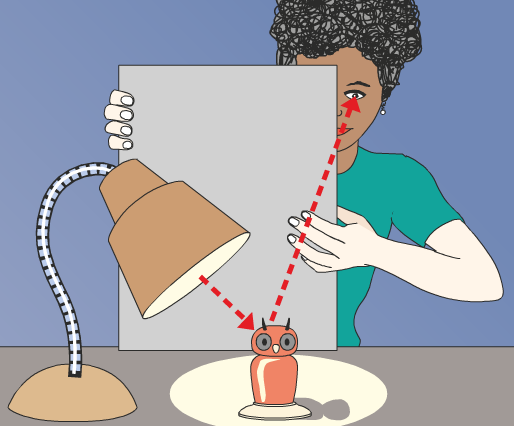
\includegraphics[scale=0.6]{bilan2}
}
\end{mybilan}


\begin{myexos}
	\begin{multicols}{2}
	
		\begin{itemize}
			\item \exo{2}{132}
			\item \exo{8}{133}
			\item \exo{14}{134}
		\end{itemize}
	
	\end{multicols}
\end{myexos}


\section{Des gaz dans l'eau}

\begin{myact}{3 page 126}
	\begin{enumerate}
		\item Au début de l'expérience le tube à essais contient de l'eau.\pause
		\item Au cours de l'expérience, dans le tube à essais des bulles apparaissent et le niveau de l'eau diminue.\pause
		\item Le bain-marie est à \num{57.6} °C.\pause
		\item Non il n'est pas nécessaire de faire beaucoup chauffer l'eau pétillante pour en récupérer le gaz.\pause
		\item Au cours de l'expérience, l'eau des tubes à essais est remplacée par du gaz.\pause
		\item Le gaz dégagé est récupéré par déplacement d'eau car il prend la place de l'eau contenue dans le tube à essais.\pause
		\item Pour récupérer le gaz contenu dans le l'eau pétillante on peut l'agiter  ou la chauffer.
	\end{enumerate}
\end{myact}

\begin{mybilan}
	
		Au moment de la \kw{pleine Lune}, il peut arriver que la Lune soit parfaitement alignée avec le Soleil et la Terre et passe dans le \kw{cône d'ombre} de la Terre : elle n'est plsu éclairée par le Soleil et s'assombrit, c'est l'\kw{éclipse de Lune}.

\end{mybilan}


\begin{myexos}
	\begin{multicols}{2}
		
		\begin{itemize}
			\item \exo{4}{132}
		\end{itemize}
		
	\end{multicols}
\end{myexos}

\section{Reconnaître le dioxyde de carbone}

\begin{myact}{4 page 127}
	\begin{enumerate}
		\item Le gaz prélevé dans la seringue a été extrait d'eau pétillante par déplacement d'eau.\pause
		\item Au début de l'expérience, la solution d'eau de chaux est incolore et transparente.\pause
		\item Après y avoir fait barboter le gaz l'eau de chaux s'est troublée.\pause
		\item Un précipité blanc s'est formé lors de cette expérience, donc le gaz dissous dans l'eau pétillante est du dioxyde de carbone.
	\end{enumerate}
\end{myact}

\begin{mybilan}
	\twoCol{
	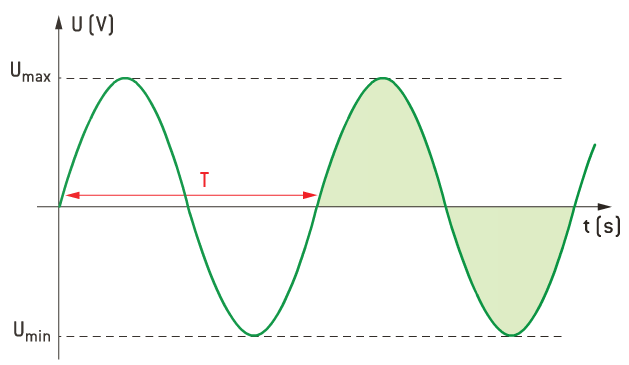
\includegraphics[scale=0.4]{bilan4}	
	\vspace*{1cm}
	\begin{enumerate}
		\item Un \kw{laser} est un faisceau de lumière d'une \kw{grande énergie} et très fin. 
		\item Le laser peut être un \kw{danger pour l'\oe il}. Il peut brûler la rétine et entrainer la cécité s'il entre dans l'\oe il.
		\item Quand on manipule un laser, quelle que soit sa puissance, il faut respecter des \kw{règles de sécurité}.
	\end{enumerate}}

\end{mybilan}

\begin{myexos}
	\begin{multicols}{2}
		
		\begin{itemize}
			\item \exo{3}{132}
			\item \exo{11}{133}
			\item \exo{12}{134} (DM ?)
			\item \exo{15}{134}
		\end{itemize}
		
	\end{multicols}
\end{myexos}

\appendix

\newpage

\section*{Correction des exercices}

\subsection*{\Exo{2}{132}}

	
	\setlength{\tabcolsep}{4pt}
	\begin{tabular}{|l|c|c|c|}
		\hline
		\textbf{Caractéristiques}                                                                            & \textbf{Solides} & \textbf{Liquides} & \textbf{Gaz} \\ \hline
		Ils ont une forme propre                                                                             & x                &                   &              \\ \hline
		\begin{tabular}[c]{@{}l@{}}Ils occupent tout le volume \\ du récipient qui les contient\end{tabular} &                  &                   & x            \\ \hline
		\begin{tabular}[c]{@{}l@{}}Au repos, leur surface libre\\  est plane et horizontale\end{tabular}     &                  & x                 &              \\ \hline
		\begin{tabular}[c]{@{}l@{}}Ils prennent la forme du \\ récipient qui les contient\end{tabular}       &                  & x                 & x            \\ \hline
		On peut les saisir avec les doigts                                                                   & x                &                   &              \\ \hline
	\end{tabular}

\subsection*{\Exo{6}{133}}

\begin{enumerate}[label=\alph*)]
	\item La surface libre d'un liquide est la surface en contact avec l'air.
	\item Le rôle du fil à plomb est d'indiquer la direction verticale et celui de l'équerre est d'indiquer la direction horizontale.
	\item On en conclu que la surface libre du liquide est horizontale.
\end{enumerate}
\subsection*{\Exo{3}{132}}

\begin{enumerate}[label=\alph*)]
	\item \twoCol{\begin{enumerate}
		\item Eau pétillante
		\item Ballon
		\item Tube à dégagement
		\item Tube à essais
		\item Eau de chaux
		\item Précipité blanc
	\end{enumerate}}
	
	\item De l'eau pétillante est placée dans un ballon. Le gaz contenu dans l'eau pétillante est extrait dans un tube à dégagement. L'autre extrémité du tube à dégagement est placée dasn un tube à essais qui contient de l'eau de chaux. Un précipité blanc se forme, le gaz dissous dans l'eau pétillante est du dioxyde de carbone.
\end{enumerate}

\subsection*{\Exo{4}{132}}

\begin{enumerate}[label=\alph*)]
	\item L'eau peut contenir des gaz \mykw{dissous}.
	\item On peut extraire un gaz d'une boisson pétillante en \mykw{agitant} ou en \mykw{chauffant} le liquide.
	\item Les gaz extraits sont récupérés par \mykw{déplacement} d'eau.
	\item Le gaz dissous dans une eau pétillante est du \mykw{dioxyde de carbone}.
	\item Pour l'identifier, on utilise le test à \mykw{l'eau de chaux}. En sa présence il se forme un \mykw{précipité blanc}.
\end{enumerate}

\subsection*{\Exo{5}{133}}

\begin{enumerate}[label=\alph*)]
	\item 

\begin{tabular}{|l|c|c|}
	\hline
	\textbf{Mot}        & \textbf{\'Etat solide} & \textbf{\'Etat liquide} \\ \hline
	pluie      &               & x              \\ \hline
	nuages     &               & x              \\ \hline
	buée       &               & x              \\ \hline
	glaciers   & x             &                \\ \hline
	mer        &               & x              \\ \hline
	neige      & x             &                \\ \hline
	givre      & x             &                \\ \hline
	brouillard &               & x              \\ \hline
	rivière    &               & x             \\ \hline
\end{tabular}

\item L'état gazeux n'est pas représenté.
\item On ne peut pas le voir car la vapeur d'eau est invisible.

\end{enumerate}

\subsection*{\Exo{8}{133}}

\begin{enumerate}[label=\alph*)]
	\item Le volume d'un gaz que l'on comprime diminue.
	\item Seringues classées par ordre croissant de compression : 2 ; 1 ; 3
\end{enumerate}

\subsection*{\Exo{11}{133}}

\begin{enumerate}[label=\alph*)]
	\item On observe que l'eau de chaux se trouble.
	\item On peut conclure que l'air expiré par Marine contient du dioxyde de carbone.
\end{enumerate}

\subsection*{\Exo{14}{134}}
\begin{enumerate}[label=\alph*)]
	\item Le contenu du flacon supérieur est devenu roux.
	\item Lorsque la coupelle a été enlevée le gaz présent dans le flacon du dessous s'est étendu pour occuper l'espace du flacon du haut.
\end{enumerate}

\subsection*{\Exo{15}{134}}
\begin{enumerate}[label=\alph*)]
	\item Le ballon gonfle rapide car l'eau a été <<renforcée en gaz de la source>>.
	\item Le gaz présent dans cette eau minérale est du dioxyde de carbone.
	\item Pour le mettre en évidence on peut faire le test de reconnaissance à l'eau de chaux.
\end{enumerate}
\end{document}]